\documentclass[]{standalone}
%\documentclass[onecolumn,journal]{IEEEtran}
%\documentclass[a4paper]{article}

%\pagestyle{empty}

%\usepackage[papersize={6cm,5cm},margin={1pt,1pt,1pt,1pt}]{geometry}

\usepackage{amsmath}
%\def\xcolorversion{2.00}
%\def\xkeyvalversion{1.8}

%\usepackage[version=0.96]{pgf}
%\usepackage{graphicx}
\usepackage{tikz}
\usetikzlibrary{arrows,shapes,backgrounds}
%% The amssymb package provides various useful mathematical symbols
\usepackage{amssymb}
%% The amsthm package provides extended theorem environments
 \usepackage{amsthm}
 \usepackage{mathrsfs}
 \usetikzlibrary{fadings,shadows}

%\usepackage{verbatim}
%\usepackage[latin1]{inputenc}


%\usepgflibrary{shapes.symbols}    
%\usepgflibrary[shapes.symbols]    
%\usetikzlibrary{shapes.symbols}  
%\usetikzlibrary[shapes.symbols]  


\begin{document}

% \begin{figure}
% \centering
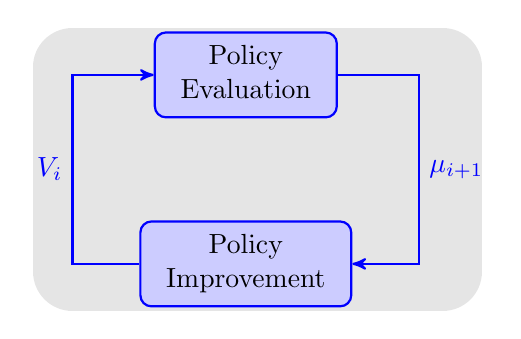
\begin{tikzpicture}[>=stealth']
	
%\tikzfading[name=arrowfading, top color=transparent!0, bottom color=transparent!95]
%\tikzset{arrowfill/.style={top color=red!20, bottom color=red, general shadow={fill=black}}}
%\tikzset{arrowstyle/.style={draw=red,arrowfill, <->, rotate=90, double arrow, minimum height=1.3cm, minimum width=3.0, double arrow, double arrow head extend=.2cm,}}
%  \tikzstyle{every label}=[red]
%  
%  \begin{scope}
\node [rectangle, draw=blue, thick, 
                        fill=blue!20, text centered,
                        rounded corners] (sys1) at (0,1.2) {\begin{tabular}{c}Policy\\ Evaluation\end{tabular}};
\node [rectangle, draw=blue, thick, 
                        fill=blue!20, text centered,
                        rounded corners] (sys2) at (0,-1.2) {\begin{tabular}{c}Policy\\ Improvement\end{tabular}};
%                        
%\node [rectangle, draw=blue, thick, 
%                        fill=blue!20, text centered,
%                        rounded corners, text width=3cm] (sys3) at (0,-3.7) {\Large Dynamic uncertainty};
%
%%\draw [<->,very thick,blue] (sys2) to (sys3);
%
%
%%    \node [draw, rectangle,  text width=3cm, text height=1cm, anchor=base] (sys1) {{\Large system 1}};
%%    \node [draw, rectangle, below of=sys1,  text width=3cm] (sys2) {{\Large system 2}};   
%%
%%
%%   \draw [->]   (sys1)  |- (sys2);
%%%        \draw [->]   (sys2)  |- (sys1);
\draw [->,thick, blue] (sys1) to node[text centered, above]{}(2.2,1.2) to node[text centered, right]{$\mu_{i+1}$}(2.2,-1.2) to  (sys2);
\draw [->,thick,blue] (sys2) to node[text centered, below]{}(-2.2,-1.2) to node[text centered, left] {$V_i$}(-2.2,1.2) to (sys1);
%%\draw [->] (-2.5,1.6) to [yshift=6](sys1);
%  \end{scope}
%  
%  \node[draw,double arrow,arrowfill,arrowstyle] at (0,-2.4){};
%
 \begin{pgfonlayer}{background}
    \filldraw [line width=10mm,join=round,black!10]
      (-2.2, 1.3)  rectangle (2.5, -1.3);
  \end{pgfonlayer}
  
\end{tikzpicture}
% \end{figure}


\end{document}